% Options for packages loaded elsewhere
\PassOptionsToPackage{unicode}{hyperref}
\PassOptionsToPackage{hyphens}{url}
%
\documentclass[
]{article}
\usepackage{amsmath,amssymb}
\usepackage{iftex}
\ifPDFTeX
  \usepackage[T1]{fontenc}
  \usepackage[utf8]{inputenc}
  \usepackage{textcomp} % provide euro and other symbols
\else % if luatex or xetex
  \usepackage{unicode-math} % this also loads fontspec
  \defaultfontfeatures{Scale=MatchLowercase}
  \defaultfontfeatures[\rmfamily]{Ligatures=TeX,Scale=1}
\fi
\usepackage{lmodern}
\ifPDFTeX\else
  % xetex/luatex font selection
\fi
% Use upquote if available, for straight quotes in verbatim environments
\IfFileExists{upquote.sty}{\usepackage{upquote}}{}
\IfFileExists{microtype.sty}{% use microtype if available
  \usepackage[]{microtype}
  \UseMicrotypeSet[protrusion]{basicmath} % disable protrusion for tt fonts
}{}
\makeatletter
\@ifundefined{KOMAClassName}{% if non-KOMA class
  \IfFileExists{parskip.sty}{%
    \usepackage{parskip}
  }{% else
    \setlength{\parindent}{0pt}
    \setlength{\parskip}{6pt plus 2pt minus 1pt}}
}{% if KOMA class
  \KOMAoptions{parskip=half}}
\makeatother
\usepackage{xcolor}
\usepackage[margin=1in]{geometry}
\usepackage{graphicx}
\makeatletter
\def\maxwidth{\ifdim\Gin@nat@width>\linewidth\linewidth\else\Gin@nat@width\fi}
\def\maxheight{\ifdim\Gin@nat@height>\textheight\textheight\else\Gin@nat@height\fi}
\makeatother
% Scale images if necessary, so that they will not overflow the page
% margins by default, and it is still possible to overwrite the defaults
% using explicit options in \includegraphics[width, height, ...]{}
\setkeys{Gin}{width=\maxwidth,height=\maxheight,keepaspectratio}
% Set default figure placement to htbp
\makeatletter
\def\fps@figure{htbp}
\makeatother
\usepackage{soul}
\setlength{\emergencystretch}{3em} % prevent overfull lines
\providecommand{\tightlist}{%
  \setlength{\itemsep}{0pt}\setlength{\parskip}{0pt}}
\setcounter{secnumdepth}{-\maxdimen} % remove section numbering
\ifLuaTeX
  \usepackage{selnolig}  % disable illegal ligatures
\fi
\IfFileExists{bookmark.sty}{\usepackage{bookmark}}{\usepackage{hyperref}}
\IfFileExists{xurl.sty}{\usepackage{xurl}}{} % add URL line breaks if available
\urlstyle{same}
\hypersetup{
  pdftitle={A Practical Guide to the Bayesian Hamiltonian Monte Carlo Method},
  pdfauthor={ Spencer Miller, fcas, maaa \& Kenny Smart, fcas, maaa },
  hidelinks,
  pdfcreator={LaTeX via pandoc}}

\title{A Practical Guide to the Bayesian Hamiltonian Monte Carlo Method}
\author{\\
Spencer Miller\textsc{, fcas, maaa} \& Kenny Smart\textsc{, fcas,
maaa}\\}
\date{2025-09-22}

\begin{document}
\maketitle
\begin{abstract}
This paper seeks to provide a practical guide to leveraging Bayesian
methods, as well as a discussion on behavioral economics as a motivating
force.
\end{abstract}

\textbf{Keywords} --- Bayesian, Monte Carlo, Markov Chain, MCMC,
Hamiltonian, Stan, Forecasting, Predictions, Behavioral Economics

\hypertarget{introduction}{%
\section{1. Introduction}\label{introduction}}

A lot has been written in the actuarial literature about Bayesian
methods over the last few decades; few of which are still part of
current exam syllabi. While these papers provide a thorough explanation
of the process, the math can seem overly complex even to an experienced
actuary. The purpose of this paper is twofold. First, we want to provide
actuaries with the \emph{basic} understanding of what goes on behind the
scenes of a Bayesian model without getting bogged down in the math.
Second, we want to champion the continued inclusion of these topics in
exam syllabi in the future.

While we believe this paper is beneficial to everyone in the profession,
we view the following as the target audience:

\begin{itemize}
\tightlist
\item
  An actuary who has finished exams a few years ago and wants to ease
  their way into Bayesian methods.
\item
  An actuary who occassionaly finds their estimates to be out of line
  with results with no discernible reason.
\item
  An actuary interested in learning about Bayesian methods but finds the
  math too onerous or intimidating.
\item
  An actuary with limited data.
\end{itemize}

In Section 2, we give a brief lesson in behavioral economics and
highlight potential biases that are relevant to the actuarial
profession.

In Section 3, we review a few common methods of making predictions and
examining their strengths and weaknesses.

In Section 4, we give a primer on the basics of Bayesian methods.

In Section 5, we use a real-life example to show how the underlying
biases in Section 2 can impact some of the prediction methods from
Section 3 and how using Bayesian methods can provide a more realistic
range of reasonable estimates.

In Section 6, we provide the reader with additional resources to further
explore these topics.

\hypertarget{a-lesson-in-behavioral-economics}{%
\section{2. A Lesson in Behavioral
Economics}\label{a-lesson-in-behavioral-economics}}

When making predictions, people often rely on heuristics. While these
are typically useful from an evolutionary standpoint, they can
``\ldots{} lead to systematic and predictable errors''. Below is a
non-exhaustive list of possible factors at play when making actuarial
predictions along with key examples (Tversky \& Kahnemann).

\hypertarget{insensitivity-to-sample-size}{%
\subsection{2.1 Insensitivity to sample
size}\label{insensitivity-to-sample-size}}

If tasked with estimating the likelihood of a particular result, people
tend to base their estimate on the sample's similarity to the
population's likelihood, regardless of sample size.

For example, subjects were given the following problem:

\begin{quote}
A certain town is served by two hospitals. In the large hospital about
45 babies are born each day, and in the smaller hospital about 15 babies
are born each day. As you know, about 50\% of all babies are boys. The
exact percentage of baby boys, however, varies from day to day.
Sometimes it may be higher than 50\%, sometimes lower.

For a period of one year, each hospital recorded the days on which more
than 60\% of the babies born were boys. Which hospital do you think
recorded more such days?

\begin{itemize}
\item
  The larger hospital
\item
  The smaller hospital
\item
  About the same (i.e., within 5\% of each other)
\end{itemize}
\end{quote}

The majority of subjects said the numbers of days would be about the
same, while the minority of subjects were split evenly between the
larger and smaller hospitals. According to sampling theory, there will
be more such days in the smaller hospital since smaller populations
generally experience higher variation.

For a more salient example, consider the actuary's task of estimating
the prospective loss ratio for a given book of business when they only
have two years of data. If the industry and historical loss ratios for
that exposure are both consistently in the 75-80\% range, you might
expect the prospective loss ratio for your book and the industry to be
similar. However, the volatility in loss ratios will be greater for your
book than for the industry.

\hypertarget{insensitivity-to-the-prior-probability-of-outcomes}{%
\subsection{2.2 Insensitivity to the prior probability of
outcomes}\label{insensitivity-to-the-prior-probability-of-outcomes}}

When making a judgment of whether item X belongs to either class A or
class B, people will assign it to the class in which the description of
item X matches the stereotype of the class, despite the relative
likelihood of each class.

For example, when subjects were tasked with evaluating the likelihood of
whether a randomly sampled person out of a pool of 30 engineers and 70
lawyers was a lawyer or an engineer, subjects correctly identified the
relative likelihoods. However, when a description of the randomly
sampled person was introduced, subjects ``evaluated the likelihood that
a particular description belonged to an engineer rather than to a lawyer
\ldots{} with little or no regard for the prior probabilities of the two
outcomes.'' Under this new condition, subjects estimated the likelihood
to be 50/50.

\hypertarget{misconception-of-chance}{%
\subsection{2.3 Misconception of chance}\label{misconception-of-chance}}

People will expect even a short sample of random events to ``look
random.'' For example, when shown two sets of a random sequences of coin
tosses, subjects will judge ``HTHTTH'' to be more likely than
``HHHTTT'', despite the true sets being equally likely.

For an example from our profession, consider the task of selecting trend
rates. While we try to incorporate external information in our
selections (hard versus soft market, inflation, changes in business
practices, etc.), there will always be a tendency to ``eyeball'' trend
lines - even when the data points have no clear trend.

While we would like to believe actuaries would be immune to this
particular bias, even experienced research psychologists were prone to
believing ``\ldots{} small sample sizes were''highly representative of
the populations from which they are drawn.''

\hypertarget{insensitivity-to-predictive-accuracy}{%
\subsection{2.4 Insensitivity to predictive
accuracy}\label{insensitivity-to-predictive-accuracy}}

When making predictions, studies show that when given only a favorable
or unfavorable description of something, subjects' predictions were
``insensitive to the reliability of the description.'' In other words,
people can take a description at face value, with little regard to the
credibility of the description.

Consider the following example. You are tasked with estimating the
average ultimate severity of claims occurring during the upcoming policy
year. The recently hired risk manager tells you that there are new
post-loss measures being put in place that will reduce the potential of
large claims. Taking the risk manager's assessment of the new claims
handling process on faith could lead to deficient estimates.

\hypertarget{misconceptions-of-regression}{%
\subsection{2.6 Misconceptions of
Regression}\label{misconceptions-of-regression}}

This is more commonly referred to as ``regression to the mean.'' If we
observe a string of higher than average values within a known
distribution, one would expect lower than average values in the next few
observations. However, studies show that many subjects do not always
recognize this phenomenon. They can either fail to believe regression is
applicable in their specific scenario or they might ``invent spurious
causal explanations.''

\hypertarget{anchoring}{%
\subsection{2.7 Anchoring}\label{anchoring}}

Suppose you're in charge of providing a loss forecast for the upcoming
accident year and have been doing so for a few years. When making your
selection, you are acutely aware of the estimated you provided last
year. This prior estimate might be ``anchoring'' your estimate of the
prospective year. While that may not be a bad thing, the issue arises
when there is insufficient adjustment to the anchoring value.

In one study, subjects were tasked with estimating the percentage of
African countries in the United Nations. However, before making their
estimate, the subjects were asked to spin a wheel with numbers from 0 to
100. The subjects had to adjust upwards or downwards from this starting
value. The median estimate for those with a starting value of 10 was
25\% compared to 45\% for those with a starting value of 65.

\hypertarget{a-review-of-prediction-methods}{%
\section{3. A Review of Prediction
Methods}\label{a-review-of-prediction-methods}}

The ``actuarial central estimates'' are'' is a cornerstone of our
profession. It reflects the culmination of years of studying and
practice. For a lot of our work, it's all that is typically required.
After all, we're seen as the experts and you'd be hard-pressed to find
an end user of our work that is as concerned about confidence levels as
we are.

But as we each have likely missed the mark on some projection at some
point in our careers, it is worth reflecting on those misses. Were they
due to chance (e.g., process risk), did we fail to adequately capture
possible alternatives (e.g., parameter risk), or was there some
underlying bias that caused us to see a trend that wasn't actually
there.

Before we go over the commonly used prediction methods, a refresher on
types of risk is required (Meyers):

\begin{itemize}
\item
  Process Risk: Average variance of the outcomes from the expected
  results.
\item
  Parameter Risk: Variance due to the many possible parameters.
\item
  Model Risk: The risk that one did not select the right model.
\end{itemize}

\hypertarget{frequentist-methods}{%
\subsubsection{3.1 Frequentist Methods}\label{frequentist-methods}}

\hypertarget{bayesian-methods}{%
\subsubsection{3.2 Bayesian Methods}\label{bayesian-methods}}

\hypertarget{basics-of-bayesian-mcmc}{%
\section{4. Basics of Bayesian MCMC}\label{basics-of-bayesian-mcmc}}

Before we get into the Hamiltonian Monte Carlo method, we provide a
brief overview of Bayesian MCMC.

\begin{itemize}
\item
  A \textbf{Markov process} is a random process for which the future
  depends only on the present state. For example, the outcome of rolling
  a die does not depend on the previous roll.
\item
  \textbf{Monte Carlo} methods use random sampling to approximate an
  outcome. Continuing the die roll example, you could replicate the
  outcome of a single roll \(r\) by generating a random value \(u\)
  from\\
  the distribution \emph{U} \textasciitilde{} Uniform{[}0,1{]}, where
  \(r=\)\(\lceil\)\(6u\)\(\rceil\).
\item
  \textbf{Bayesian statistics} is an approach to data analysis based on
  Bayes' theorem, where available knowledge about parameters in a
  statistical model is updated with the information in observed data. In
  our example, let's assume that the die is not fair (unbeknownst to us)
  with a distribution equal to \(Prob(r = i) = i/21\) and that we have
  observed the following rolls: \(y\) = \{3, 4, 5, 6, 4, 3, 5, 4, 2\}.

  Using a Bayesian approach, we have three components:

  \begin{itemize}
  \item
    \emph{Likelihood function}: This is the parametric form of our data,
    \(p(y|\theta)\), given a set of parameters, \(\theta\).
  \item
    \emph{Prior distribution}: This is our belief of the distribution of
    our parameters prior to seeing the data, \(p(\theta)\). In this
    case, we might assume that the die is fair: \(p(\theta) = 1/6\).
  \item
    \emph{Posterior distribution}: The result of updating our prior
    belief about the parameters given the data,
    \(p(\theta|y) \propto p(\theta) * p(y|\theta)\).
  \end{itemize}
\end{itemize}

This process can be done using \textbf{Stan}, an open-source software,
via common coding languages (e.g., python and R). In this paper, we
leverage the RStan package, though there are numerous other packages
that can be used.

\begin{itemize}
\tightlist
\item
  Need to discuss the key parameters (thin, chains, etc.).
\item
  Discuss sampling method: Gibbs vs Metropolis Hastings vs Hamiltonian
  Monte Carlo
\end{itemize}

Applying this process to our loaded die example: \emph{Kenny to
complete}

\hypertarget{an-example-in-action}{%
\section{5. An Example in Action}\label{an-example-in-action}}

For our example, let's assume you are tasked with estimating the
expected frequency of earthquakes over 6.0 magnitude for the upcoming
year (2012). You are given a dataset of prior earthquakes since 1983.

First, let's get the data we'll be using in our example. Below is the
history for the last .

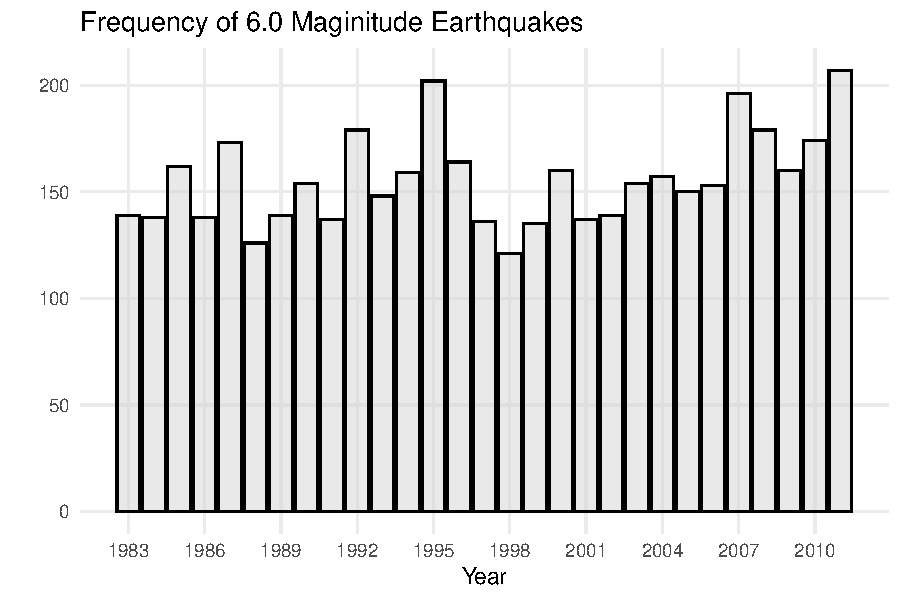
\includegraphics{C:/Users/spencer.miller/Documents/Repos/bayesian_mcmc_paper/paper_files/figure-latex/data_by_year-1.pdf}

In the simplest case you may decide given the recent trend, that the
five-year average is the best approximation of future frequency. In this
case, your selected frequency is 183 (``Point Estimate'').

Your next logical step might be to add some process risk around your
estimate by fitting a distribution to the data. Based on an examination
of the data, you decide to model frequency using the Poisson
distribution with lambda = 183.

After running 10,000 simulations with your selected distribution, you're
left with a central estimate of 183. Not surprisingly, this is
essentially the same as your point estimate. However, you now have a
predictive distribution.

Another possible step would be to layer in parameter risk since we might
not be convinced of our selected lambda. You decide on letting lambda
follow a chi-square distribution with degrees of freedom equal to your
point estimate.

After running another 10,000 simulations, you're left with a central
estimate of 183. Even though we let lambda vary, the result is still
quite close to the point estimate.

But as we discussed earlier, there are a few problems with just relying
on our data:

\begin{itemize}
\tightlist
\item
  The sample size is on the low end (n = 29).
\item
  Regression to the mean.
\item
  It might look like there is a ``new normal'' but you could be seeing a
  trend where there isn't one.
\end{itemize}

How do we handle these possible biases? That's where Bayesian MCMC comes
in. We'll continue with the distribution from our parameter risk model.

After running 10,000 simulations with your selected distribution, you're
left with a central estimate of 156. Since you used a wide prior, your
result will be closer to the historical average (156) than the point
estimate (183).

Let's compare each result to the true number of earthquakes that
occurred in 2012 (133).

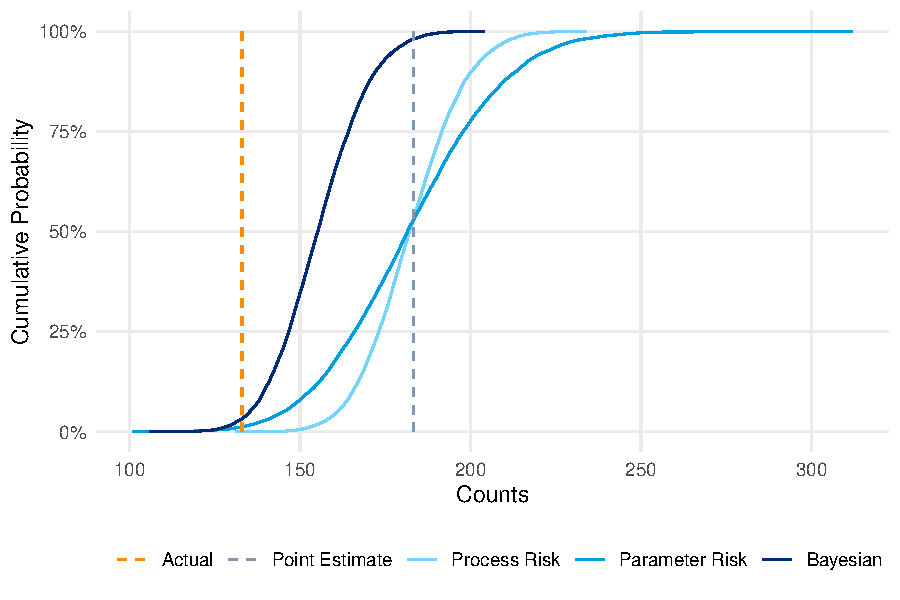
\includegraphics{C:/Users/spencer.miller/Documents/Repos/bayesian_mcmc_paper/paper_files/figure-latex/compare_true-1.pdf}

It appears that all four methods severely underestimated the true
average losses. However, if we look at the Bayesian versus the other
three, the true count is a more likely outcome. The ``true count'' is
approximately equal to the 3.3\% confidence level of our Bayesian
estimate. While this may still seem low, it is relatively close to the
prportion of counts below 133 (6.9\%).

Additionally, there are essentially no ``extreme'' values (225+) being
simulated.

With the benefit of hindsight, let's see why we overestimated the true
counts in all four methods. As it turns out, we fell prey to (at least)
two key biases:

\begin{itemize}
\tightlist
\item
  \ul{Misconception of chance}. Humans just aren't that great at
  identifying random processes. For example, a series of coin tosses
  with all heads is seen as ``less random'' than a series with
  alternating heads and tails, even though both results are equally
  likely.
\item
  \ul{Misconceptions of Regression}. As seen in the chart, the high
  average for 2007-2011 was followed by a low average in 2012-2023. This
  resulted in the new all-year average (1983-2023) being nearly
  identical to the all-year average before the rise (1983-2006).
\end{itemize}

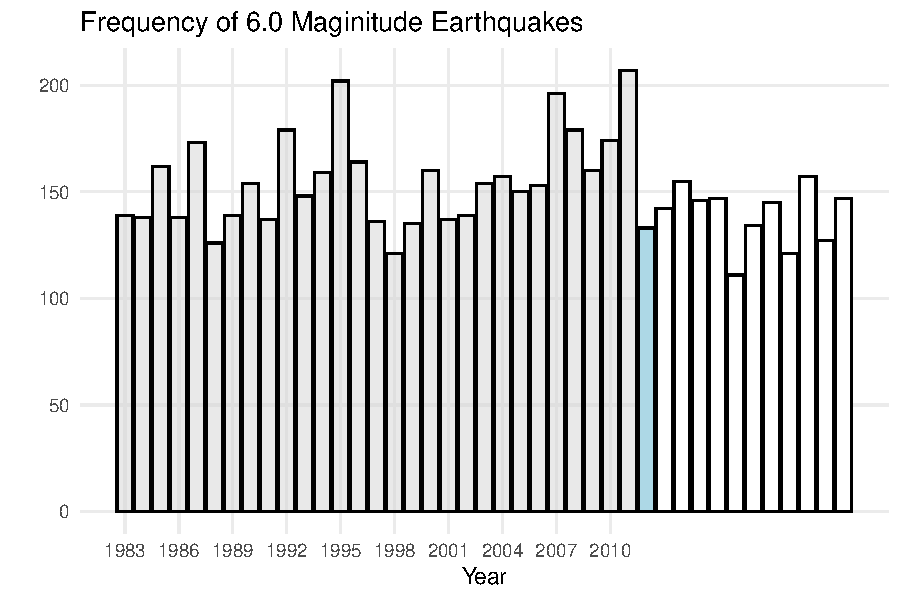
\includegraphics{C:/Users/spencer.miller/Documents/Repos/bayesian_mcmc_paper/paper_files/figure-latex/plot_full-1.pdf}

\hypertarget{supplemental-information}{%
\section{6. Supplemental Information}\label{supplemental-information}}

\hypertarget{literature-review}{%
\subsection{6.1 Literature Review}\label{literature-review}}

While our paper focused on the usage of Bayesian MCMC methods for
forecasting purposes, the methods can and have been used in other
applications. We provide a non-exhaustive list below of papers that
utilize these methods to some extent:

\begin{itemize}
\item
  Trends (Schmid)
\item
  Reserving (Meyers 2015)
\item
  Renewal Functions (Aminzadeh \& Deng)
\item
  Risk Margins (Meyers 2019)
\item
  Incorporating expert opinion into traditional reserving methods
  (Verrall)
\end{itemize}

We also believe there are several other possible applications, ranging
from the selection of development factors to estimating reserve
variability. We leave it to the reader to explore these.

\hypertarget{acknowledgements}{%
\subsection{6.2 Acknowledgements}\label{acknowledgements}}

We would like to extend our gratitude to our colleagues for their
thoughtful reviews (Rajesh Sahasrabuddhe, Molly Colleary, Alex Taggart,
and Chris Schneider).

\hypertarget{biographies-of-the-authors}{%
\subsection{6.3 Biographies of the
Authors}\label{biographies-of-the-authors}}

Spencer is a Senior Manager with Oliver Wyman Actuarial Consulting,
Inc., located in Philadelphia. He holds a Bachelor of Science from
Lebanon Valley College.

Kenny is a Senior Manager with Oliver Wyman Actuarial Consulting, Inc,
located in Chicago. He holds a Bachelor of Science degree in Actuarial
Mathematics and Statistics from the University of Pittsburgh.

\hypertarget{citations}{%
\subsection{6.4 Citations}\label{citations}}

A. Tversky, and D. Kahneman. 1974. ``Judgment Under Uncertainty:
Heuristics and Biases.'' Science 185, 1124--1131.

Aminzadeh, M.S., and Min Deng. 2022. ``Bayesian Estimation of Renewal
Function Based on Pareto-Distributed Inter-Arrival Times via an MCMC
Algorithm.'' Variance 15 (2).

Meyers, G. 2015. ``Stochastic Loss Reserving Using Bayesian MCMC
Models.'' CAS Monograph \#1.

Meyers, G. 2019. ``A Cost-of-Capital Risk Margin Formula for Nonlife
Insurance Liabilities.'' Variance 12 (2).

Sahasrabuddhe, R. 2021. ``The Single Parameter Pareto Revisited.''
Casualty Actuarial Society E-Forum, Spring 2021.

Schmid, F. 2013. ``Bayesian Trend Selection.'' Casualty Actuarial
Society E-Forum, Spring 2013.

Verrall, R. J. 2007. ``Obtaining Predictive Distributions for Reserves
Which Incorporate Expert Opinion.'' Variance 1 (1).

\hypertarget{r-packages}{%
\subsection{6.5 R Packages}\label{r-packages}}

Barrett, Tyson, Matt Dowle, Arun Srinivasan, Jan Gorecki, Michael
Chirico, Toby Hocking, Benjamin Schwendinger, and Ivan Krylov. 2025.
``Data.table: Extension of 'Data.frame`.''
\url{https://CRAN.Rproject.org/package=data.table}.

Dutang, Christophe, and Arthur Charpentier. 2025. ``CASdatasets:
Insurance Datasets.'' \url{https://doi.org/10.57745/P0KHAG}.

Stan Development Team. 2025. ``\{RStan\}: The \{r\} Interface to
\{Stan\}.'' \url{https://mc-stan.org/}.

Wickham, Hadley. 2016. ``Ggplot2: Elegant Graphics for Data Analysis.''
\url{https://ggplot2.tidyverse.org}.

\end{document}
